% !TeX spellcheck = en_GB
\ifcsname SlidesDistr\endcsname%
\documentclass[handout,aspectratio=169]{beamer}
\else%
\documentclass[aspectratio=169]{beamer}
\fi%
\usepackage{fontspec}
\usepackage[T1]{fontenc}
\usepackage{amsmath}
\usepackage{amsfonts}
\usepackage{amssymb}
\usepackage{graphicx}
\usepackage{csquotes}
\usepackage{booktabs}
\usepackage{multicol}
\usepackage{enumerate}
\usepackage{microtype}
\usepackage[labelfont=bf,font={small}]{caption}
\usepackage{hyperref}
\usepackage{booktabs}
\usepackage{subcaption}
\usepackage{fancyhdr}
\usepackage{pdfpages}

\defaultfontfeatures{Mapping=tex-text}
\newfontfamily\symbolfont{Symbola}

\usepackage[sorting=none]{biblatex}
\addbibresource{../bibliography.bib}

\author{Andreas Stöckel}

\renewcommand{\vec}[1]{{\mathbf{#1}}}
\newcommand{\mat}[1]{{\mathbf{#1}}}

% Tango color palette
\definecolor{butter1}{HTML}{FCE94F}
\definecolor{butter2}{HTML}{EDD400}
\definecolor{butter3}{HTML}{C4A000}
\definecolor{orange1}{HTML}{FCAF3E}
\definecolor{orange2}{HTML}{F57900}
\definecolor{orange3}{HTML}{CE5C00}
\definecolor{chocolate1}{HTML}{E9B96E}
\definecolor{chocolate2}{HTML}{C17D11}
\definecolor{chocolate3}{HTML}{8F5902}
\definecolor{chameleon1}{HTML}{8AE234}
\definecolor{chameleon2}{HTML}{73D216}
\definecolor{chameleon3}{HTML}{4E9A06}
\definecolor{skyblue1}{HTML}{729FCF}
\definecolor{skyblue2}{HTML}{3465A4}
\definecolor{skyblue3}{HTML}{204A87}
\definecolor{plum1}{HTML}{AD7FA8}
\definecolor{plum2}{HTML}{75507B}
\definecolor{plum3}{HTML}{5C3566}
\definecolor{scarletred1}{HTML}{EF2929}
\definecolor{scarletred2}{HTML}{CC0000}
\definecolor{scarletred3}{HTML}{A40000}
\definecolor{aluminium1}{HTML}{EEEEEC}
\definecolor{aluminium2}{HTML}{D3D7CF}
\definecolor{aluminium3}{HTML}{BABDB6}
\definecolor{aluminium4}{HTML}{888A85}
\definecolor{aluminium5}{HTML}{555753}
\definecolor{aluminium6}{HTML}{2E3436}

\definecolor{violet}{HTML}{AA305C}
\definecolor{uwyellow}{HTML}{FDD433}
\definecolor{background}{HTML}{F9F9F6}
\definecolor{text}{HTML}{000000}

\definecolor{uweng1}{HTML}{D1B2EE}
\definecolor{uweng2}{HTML}{BF33DE}
\definecolor{uweng3}{HTML}{8001B3}
\definecolor{uweng4}{HTML}{56048A}

\setbeamercolor{title}{fg=violet}
\setbeamercolor{frametitle}{fg=black}
\setbeamercolor{structure}{fg=aluminium5}
\setbeamercolor{normal text}{fg=text}

\setbeamertemplate{navigation symbols}{}
\setbeamertemplate{footline}[frame number]


\newcommand{\hl}[1]{\colorbox{uwyellow}{{\textbf{#1}}}}

\newcommand{\ColorRect}[3]{{\color{#1}\rule{#2}{#3}}}
\setbeamertemplate{headline}{\ColorRect{black}{\textwidth}{4pt}\newline\ColorRect{uweng1}{0.25\textwidth}{4pt}\ColorRect{uweng2}{0.25\textwidth}{4pt}\ColorRect{uweng3}{0.25\textwidth}{4pt}\ColorRect{uweng4}{0.25\textwidth}{4pt}}

\newcommand{\MakeTitle}{
	\vspace{0.5cm}
	{\textbf{\inserttitle}}\\[0.5cm]
	\insertauthor\\[0.5cm]
	\insertdate\\
	\vspace{2cm}
 	\includegraphics[width=0.5\textwidth]{../assets/uwlogo_eng.pdf}
}

\newcommand{\handwritingframe}{%
	\begin{frame}
		\begin{columns}
			\column{\paperwidth}
			
\includegraphics{../assets/handwriting_lines.pdf}
		\end{columns}
	\end{frame}	
}



\usepackage{ragged2e}

\date{February 25 \& 27, 2020}
\title{SYDE 556/750 \\ Simulating Neurobiological Systems \\ Lecture 8: Learning}

\begin{document}
	
	\begin{frame}{}
		\vspace{0.5cm}
		\begin{columns}[c]
			\column{0.6\textwidth}
			\MakeTitle
			\column{0.4\textwidth}
			\includegraphics[width=\textwidth]{media/laurentius_de_voltolina_001_small.jpg}
		\end{columns}
	\end{frame}

	\begin{frame}{Supervised Learning}
		\centering
		\includegraphics[scale=0.95]{media/learning_example_supervised.pdf}
	\end{frame}

	\begin{frame}{Supervised Learning -- Training}
		\centering
		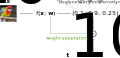
\includegraphics[scale=0.95]{media/learning_example_supervised_2.pdf}
	\end{frame}

	\begin{frame}{Supervised Learning -- Inference}
		\centering
		
\includegraphics[scale=0.95]{media/learning_example_supervised_3.pdf}
	\end{frame}

	\begin{frame}{Gradient Descent -- Example}
		\centering%
		\includegraphics<1>[width=\textwidth]{media/gradient_descent_poly_example_00.pdf}%
		\includegraphics<2>[width=\textwidth]{media/gradient_descent_poly_example_01.pdf}%
		\includegraphics<3>[width=\textwidth]{media/gradient_descent_poly_example_02.pdf}%
		\includegraphics<4>[width=\textwidth]{media/gradient_descent_poly_example_03.pdf}%
		\includegraphics<5>[width=\textwidth]{media/gradient_descent_poly_example_04.pdf}%
		\includegraphics<6>[width=\textwidth]{media/gradient_descent_poly_example_05.pdf}%
		\includegraphics<7>[width=\textwidth]{media/gradient_descent_poly_example_06.pdf}%
		\includegraphics<8>[width=\textwidth]{media/gradient_descent_poly_example_07.pdf}%
		\includegraphics<9>[width=\textwidth]{media/gradient_descent_poly_example_08.pdf}%
		\includegraphics<10>[width=\textwidth]{media/gradient_descent_poly_example_09.pdf}%
		\includegraphics<11>[width=\textwidth]{media/gradient_descent_poly_example_10.pdf}%
	\end{frame}

	\begin{frame}{Supervised Learning -- Generalisation}
		\centering%
		\includegraphics<1>[width=\textwidth]{media/gradient_descent_poly_example_gt.pdf}%
	\end{frame}

	\begin{frame}{Learning Decoders and Learning Weights}
		\begin{columns}[T]
			\column{0.5\textwidth}
			\centering			
			\hl{Learning Decoders} (Delta Rule)\\[0.25cm]
			\includegraphics{media/pes_network_a.pdf}\\[-0.5cm]
			$$\Delta d_i = - \eta a_i(\vec x) \underbrace{\big(y(t) - y^\mathrm{d}(t)\big)}_{\epsilon(t)}$$
			\column{0.5\textwidth}
			\centering			
			\hl{Learning Weights} (PES Rule)\\[0.25cm]
			\includegraphics{media/pes_network_b.pdf}\\[-0.5cm]
			$$\Delta w_{ij} = - \eta a_i(\vec x) \Big(\alpha_j \langle \vec e_j, \vec \epsilon(t) \rangle \Big)$$
		\end{columns}
	\end{frame}

	\begin{frame}{Example: Learning Functions (I)}
		\centering
		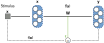
\includegraphics[scale=1.0]{media/learning_network.pdf}
	\end{frame}

	\begin{frame}{Example: Learning Functions (II)}
		\centering
		Communication Channel $f(x) = x$\\[0.125cm]
		\includegraphics[width=\textwidth]{media/pes_communication_channel_example.pdf}\\[0.125cm]
		\begin{overlayarea}{\textwidth}{0.5cm}
			\centering
		\end{overlayarea}
	\end{frame}

	\begin{frame}{Example: Learning Functions (III)}
		\centering
		Square $f(x) = x^2$\\[0.125cm]
		\includegraphics[width=\textwidth]{media/pes_square_example.pdf}\\[0.125cm]
		\begin{overlayarea}{\textwidth}{0.5cm}
			\centering
			\only<2->{\hl{Works, but learns more slowly!$\vphantom{\epsilon(t)}$}}
			\only<2->{\hl{Where is the error signal $\epsilon(t)$ coming from?}}
		\end{overlayarea}
	\end{frame}

	\begin{frame}{Example: Classical Conditioning (I)}
		\centering
		Before conditioning:\\[0.125cm]
		\includegraphics{media/classical_conditioning_a.pdf}\\[0.5cm]
		After conditioning:\\[0.125cm]
		\includegraphics{media/classical_conditioning_b.pdf}\\[0.5cm]
		\ImageSources{Images adapted from \href{https://commons.wikimedia.org/wiki/File:Classical_conditioning_-_extinction.svg}{Wikimedia}.}
	\end{frame}

	\begin{frame}{Example: Classical Conditioning (II)}
		\centering
		\vspace{0.25cm}
		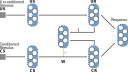
\includegraphics{media/conditioning_network.pdf}
	\end{frame}

	\begin{frame}{Example: Classical Conditioning (III)}
		\centering
		\includegraphics[width=\textwidth]{media/classical_conditioning_experiment.pdf}
	\end{frame}

	\begin{frame}{Example: Adaptive Controller}
		\centering
		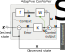
\includegraphics[height=7cm]{media/adaptive_controller.pdf}
	\end{frame}

	\begin{frame}{Unsupervised Learning}
		\centering
		\includegraphics[scale=0.95]{media/learning_example_unsupervised.pdf}
	\end{frame}
	
	\begin{frame}{Unsupervised Learning -- Training}
		\centering
		\includegraphics[scale=0.95]{media/learning_example_unsupervised_2.pdf}
	\end{frame}
	
	\begin{frame}{Unsupervised Learning -- Inference}
		\centering
		\includegraphics[scale=0.95]{media/learning_example_unsupervised_3.pdf}
	\end{frame}

	\begin{frame}{Autoencoder}
		\centering
		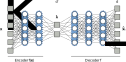
\includegraphics[width=\textwidth]{media/autoencoder.pdf}
	\end{frame}

	\videoframe{clip_variational_autoencoder}{Q1XuXwPVFko}

	\begin{frame}{PCA in Python}
		\centering
		
\includegraphics[width=\textwidth]{media/pca_code.pdf}
	\end{frame}

	\begin{frame}{PCA Example: Source Images}
		\centering
		\begin{columns}[c]
			\column{0.4\textwidth}
			\hl{Face Database}
			\begin{itemize}
				\item 84 images of 12 women\\with 7 different expressions
				\item Normalised eye location
				\item $45 \times 60$ pixels\\(2700 dimensions)
				\item Greyscale
			\end{itemize}
			\column{0.4\textwidth}
			\includegraphics[width=\textwidth]{media/face_database.pdf}
		\end{columns}
		\ImageSources{\enquote{Pain Expression Subset;} \url{http://pics.stir.ac.uk/2D_face_sets.htm}}
	\end{frame}

	\begin{frame}{PCA Example: Eigenfaces}
		\begin{columns}
			\column{0.4\textwidth}
			\centering
			\hl{Identity Basis}\\
			\includegraphics[width=0.95\textwidth]{media/eigenfaces_normal_basis.pdf}
			\column{0.4\textwidth}
			\centering
			\hl{Principal Components}\\
			\includegraphics[width=0.95\textwidth]{media/eigenfaces.pdf}
		\end{columns}		
	\end{frame}

	\begin{frame}{PCA Example: Face Spaces}
		\begin{columns}
			\column{0.5\textwidth}
			\centering
			\includegraphics[height=7.5cm]{media/eigenfaces_dim_0_1.pdf}
			\column{0.5\textwidth}
			\centering
			\includegraphics[height=7.5cm]{media/eigenfaces_dim_2_3.pdf}
		\end{columns}
	\end{frame}

	\begin{frame}{PCA Example: Sparse Vectors}
		\centering
		\includegraphics[width=\textwidth]{media/face_sparse.pdf}
	\end{frame}

	\begin{frame}{PCA Example: Modifying the Latent Space}
		\centering
		\rotatebox[origin=c]{270}{\hspace*{-6.75cm}$\leftarrow$ Smaller $\lambda_6$ \hspace{1.5cm} Larger $\lambda_6 \rightarrow$}
		\includegraphics[height=7cm]{media/face_manipulation.pdf}\\
		\hspace{0.33cm} $\leftarrow$ Smaller $\lambda_7$ \hspace{0.75cm} Larger $\lambda_7 \rightarrow$
	\end{frame}

	\begin{frame}{Limitations of PCA: Classifying Two Groups}
		\centering
		\includegraphics[width=\textwidth]{media/pca_limitations_plots.pdf}
	\end{frame}

	\begin{frame}{Limitations of PCA: Metaphorical Illustration}
		\centering
		\vspace{0.25cm}
		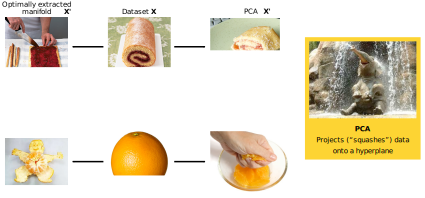
\includegraphics{media/pca_limitations.png}\\[0.25cm]
		\ImageSources{Barbara Hammer, \enquote{Maschinelles Lernen im Web}, Universität Bielefeld, WS 2014/15}
	\end{frame}

	\begin{frame}{Hebbian Learning}
		\begin{columns}
			\column{0.8\textwidth}
			{\large\justify\quotefont When an axon of cell $A$ is near enough to excite a cell $B$ and repeatedly or persistently takes part in firing it, some growth process or metabolic change takes place in one or both cells such that $A$'s efficiency, as one of the cells firing $B$, is increased.\\[0.25cm]\raggedleft\color{aluminium4} --- Donald O. Hebb, \enquote{The Organization of Behaviour}, 1949\\}
		\end{columns}
	\end{frame}

	\begin{frame}{Example: Normalised Hebbian Learning}
		\centering
		\includegraphics[width=\textwidth]{media/hebbian_learning_example.pdf}
		Learning an encoder $\vec e$, with $\| \vec e \| = 1$, 10000 steps, $\eta = 0.2 \times 10^{-4}$, $\Delta \vec e = \eta (\vec x \circ \vec e)$
	\end{frame}

	\begin{frame}{Spike-Time Dependent Plasticity}
        \centering
		\includegraphics{media/stdp.pdf}
	\end{frame}

	\begin{frame}{Conclusion}
		\begin{columns}[T]
			\column{0.5\textwidth}
			{\centering
			\hl{Supervised Learning}\\[0.25cm]}
			\begin{itemize}
				\setlength{\itemsep}{0.3cm}
				\item Find $\vec w$ such that $f(\vec x_k; \vec w) \approx \vec t_k$
				\item \emph{Hope:} $f(\vec x_k; \vec w) \approx f_\mathrm{GT}(\vec x_k)$
				\item Use gradient descent to find $\vec w$
				\item Delta, PES learning rules
				\item Modulatory synapses in the brain
			\end{itemize}
			\column{0.5\textwidth}
			{\centering
			\hl{Unsupervised Learning}\\[0.25cm]}
			\begin{itemize}
				\setlength{\itemsep}{0.25cm}
				\item Dimensionality reduction $f(\vec x_k) = \lambda_k$
				\item \emph{Hope:} latent dimensions $\vec \lambda$ are \enquote{meaningful}
				\item Autoencoders (nonlinear),\\PCA (linear)
				\item Hebbian learning $\Rightarrow$ learns PCA
			\end{itemize}
		\end{columns}
	\end{frame}

	\backupbegin

	\begin{frame}[noframenumbering]{Image sources}
		\small
		\textbf{Title slide}\\Page from \enquote{Liber ethicorum des Henricus de Alemannia}. Title: \enquote{Henricus de Alemannia con i suoi studenti} (Henricus of Germany with his students), second half of 14th century.\\From \href{https://commons.wikimedia.org/wiki/File:Laurentius_de_Voltolina_001.jpg}{Wikimedia}.
	\end{frame}

	\backupend
	
\end{document}
